\section{Human to Human Handover}

- here we talk about the dataset used for understanding human manipulation of cups with different properties, characteristics, shapes, etc.

- talk about the necessity of performing these HHI experiments 

\subsection{Experimental Scenario}

The experiments includes 4 participants, all male, with age between 25-35 years old, and academic employees. The experimental task involves grasping a cup from a table and hand it over to a subject on the opposite side that places it back in the Figure \ref{fig:epfl_dataset}.

The experiment is performed under two conditions: (i) empty cup, and (ii) cup 90\% filled with water. For each condition the experiment is repeated a minimum of 4 times per participant for each cup manipulated. There are 3 cups: red cup, plastic cup, and champagne cup. Each participant had to grasp the cups with their preferred hand (right hand for all) and there were no restriction on the type of grasp. Motion capture system (OptiTrack) recorded right-hand wrist's location for each participants as well as the cup's location. A total of 30 right-hand wrist trajectories were collected for either of the two conditions. This HHI dataset was gathered in collaboration with the High Performance Humanoid Technologies Lab (H2T) of the Karlsruher Institut für Technologie (KIT)~\footnote{\url{http://h2t.anthropomatik.kit.edu/english/index.php}} \cite{starke2019force}.

Add more details. Data was recorded at 120 Hz, the handover take around 1-3 seconds, Hence you have on average 200-300 data points for the handover trajectories.

here it is a figure illustrating the EPFL dataset.
    \begin{figure}
        \centering
        \begin{tabular}{@{}c@{}}
            \centering
            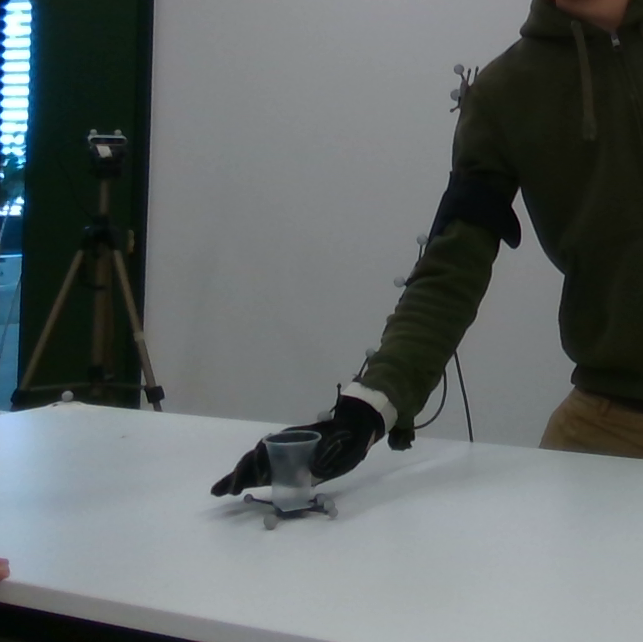
\includegraphics[width=0.225\textwidth]{Images/frame000023.png}
        \end{tabular}
        \begin{tabular}{@{}c@{}}
            \centering 
            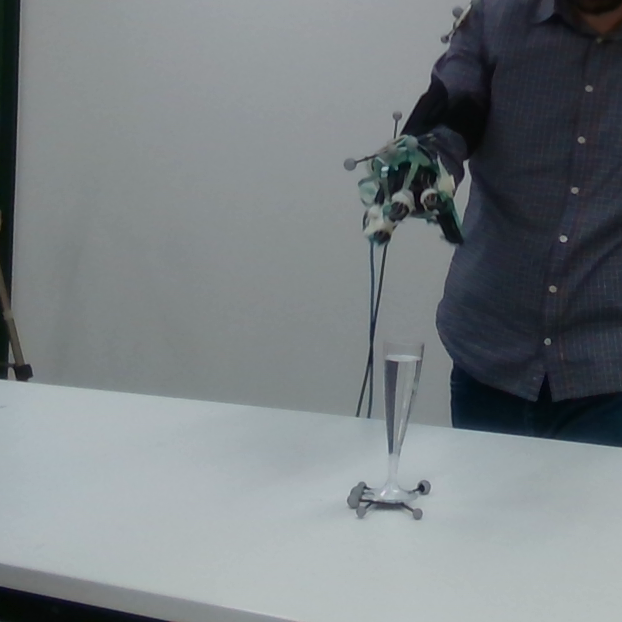
\includegraphics[width=0.224\textwidth]{Images/frame000046.png}
        \end{tabular}
        \baselineskip
        \begin{tabular}{@{}c@{}}
            \centering 
            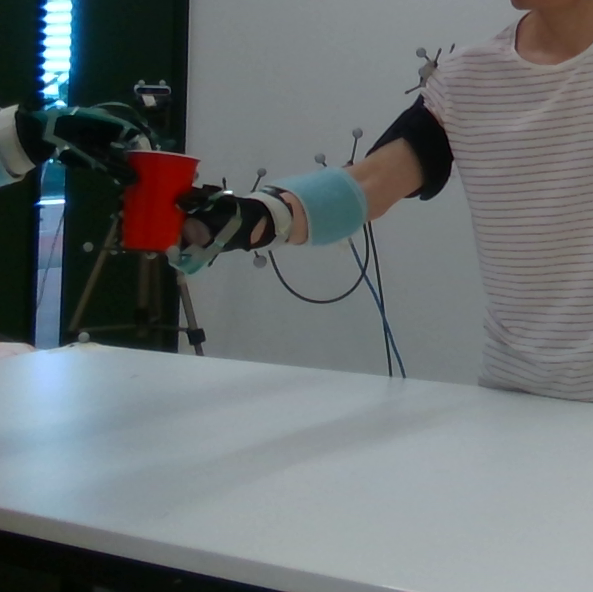
\includegraphics[width=0.226\textwidth]{Images/frame000117.png}
        \end{tabular}
        \begin{tabular}{@{}c@{}}
            \centering 
            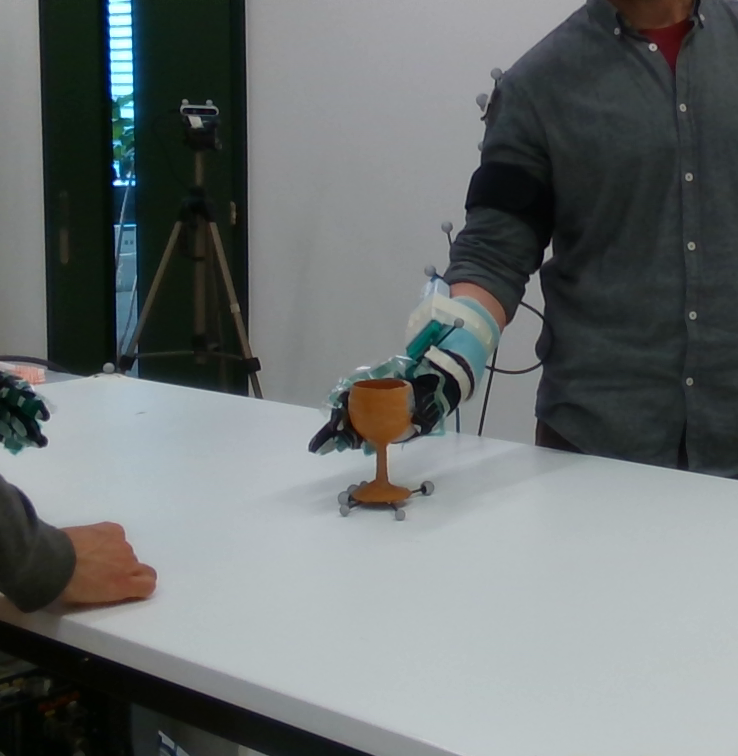
\includegraphics[width=0.223\textwidth]{Images/frame000144.png}
        \end{tabular}
        \caption{The 4 participants with the 4 cups}
        \label{fig:epfl_dataset}
    \end{figure}

\subsection{Handover Motion Analysis}

- analysis the data distance/velocity (inverse time of flight)

- analysis the data time/velocity

- mention that in the results we present two other datasets (QMUL, IST)

\subsection{Discussion}

- resume what you see from the data analysis of the human wrist

    \begin{figure}[t]
      \centering
      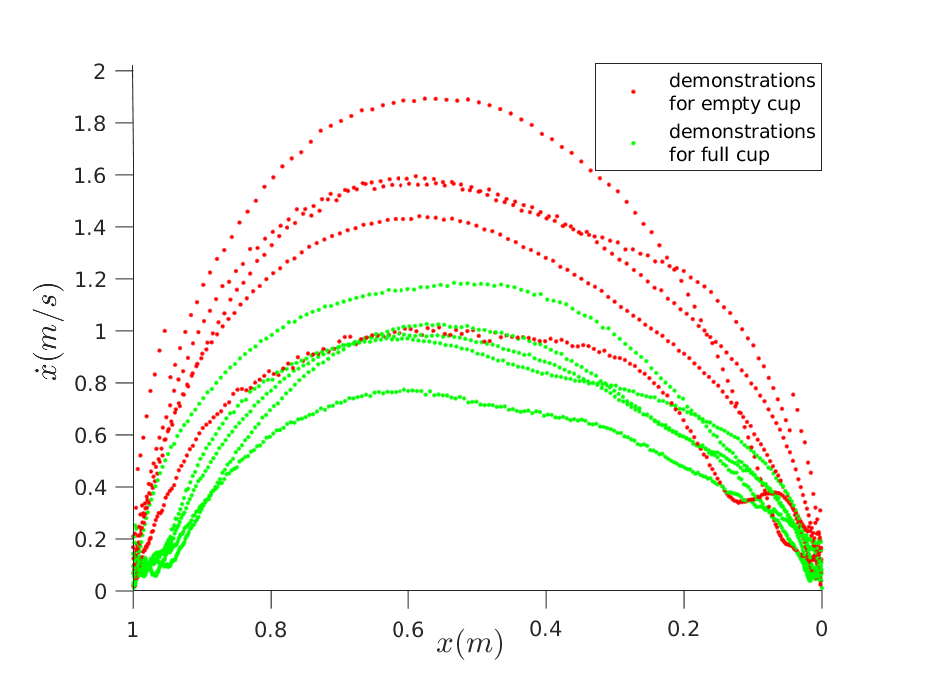
\includegraphics[width = 0.48\textwidth]{Images/vel_distance_plot.eps}
      \caption{Add legend} 
      \label{fig:vel_distance}
	\end{figure}
	
	
    \begin{figure}[t]
      \centering
      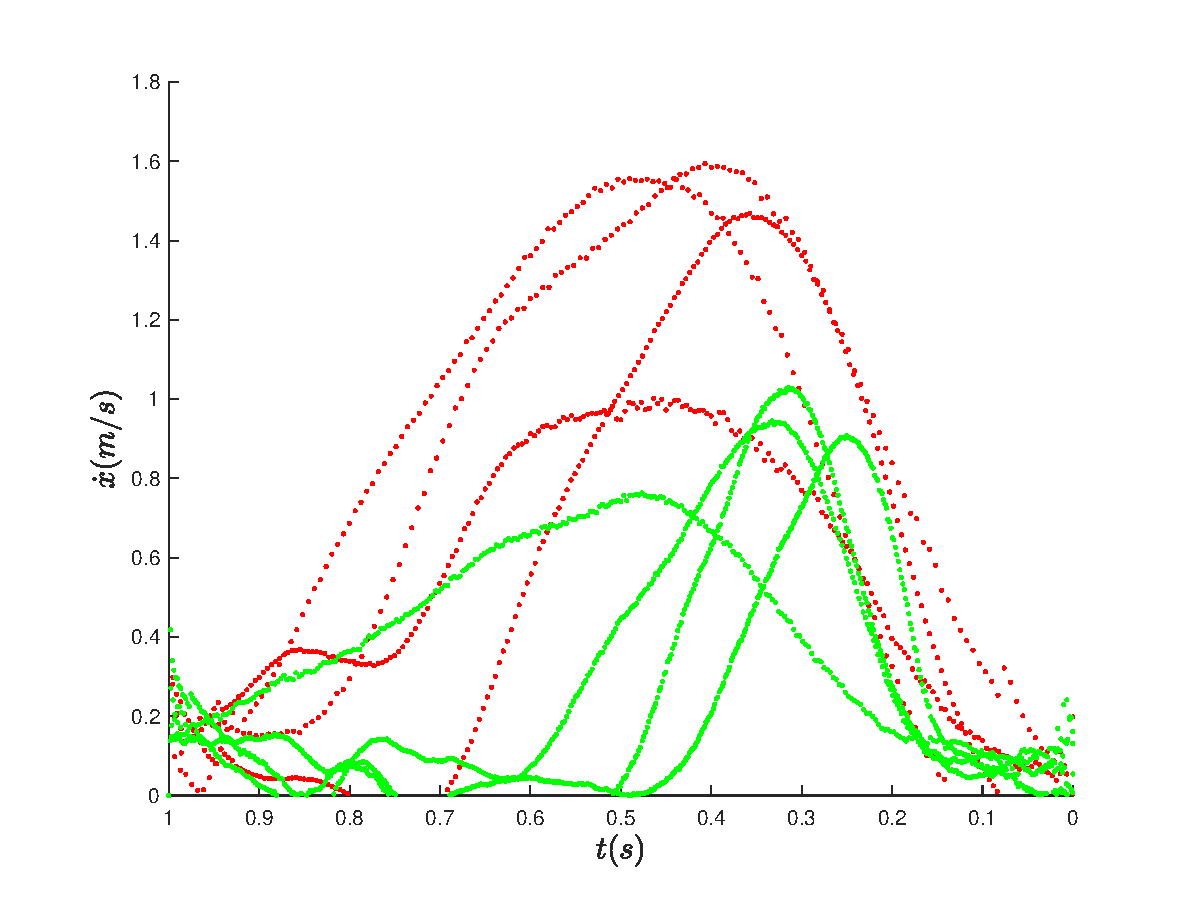
\includegraphics[width = 0.48\textwidth]{Images/vel_time_plot.eps}
      \caption{Add legend} 
      \label{fig:vel_time}
	\end{figure}
	